% vim: spelllang=fr

\documentclass[../main.tex]{subfiles}
\graphicspath{{\subfix{../Figures/Chap2/}}}
\begin{document}

\begin{itshape}
Ce deuxième chapitre porte de l'approche directe consistant en l'application d'un algorithme de détection et de suivi des cyclones tropicaux dans les modèles
comme façon de caractériser l'activité cyclonique simulée, ainsi que la façon dont les modèles représentent ces phénomènes. Un cas d'étude est présenté via
l'application du schéma de détection du CNRM à la réanalyse ERA5.
\end{itshape}

\minitoc\newpage
%--------------------------------------
\section{Tour d'horizon des techniques de détection et de suivi}\label{sec:tour_horizon_tracking}

\subsection{Schémas de détection à seuils absolus}

Les algorithmes de détection et de suivi des HTV dans les modèles consistent à identifier les points de grille qui satisfont des critères thermiques ou
dynamiques associés à un cyclone tropical. Les premiers schémas de détection étaient basés uniquement sur la MSLP et la vitesse des vents
\parencite{bengtsson_simulation_1982,broccoli_can_1990}, tandis que \cite{haarsma_tropical_1993,bengtsson_hurricanetype_1995} ajoutèrent à cela des critères sur
la vorticité ainsi qu'un diagnostique sur la présence d'un cœur chaud, dans l'optique de discriminer les perturbations tropicales de leurs homologues
extra-tropicales. \cite{wu_gcm_1992} sont les seuls, à ma connaissance, à avoir utilisé des critères supplémentaires conçus pour discriminer les perturbations
tropicales sèches via un seuil d'humidité relative, les perturbations équatoriales d'est en interdisant le vent d'est à \hPa{950} au point situé à \ang{4.5} au
nord et au sud du cyclone, ainsi que les perturbations barocliniques en bornant la vitesse du vent d'ouest à \hPa{200} au dessus du centre du cyclone à
\ms{5}. Beaucoup des traqueurs plus récents se sont concentrés sur les critères dynamiques accompagnés d'un diagnostique de cœur chaud ont depuis repris, à la
façon de \cite{haarsma_tropical_1993,bengtsson_hurricanetype_1995}. Spécifiquement, le schéma de détection employé dans \cite{bengtsson_hurricanetype_1995} est
défini par les critères suivants :
%
\begin{enumerate}
    \item\label{tracking_bengtsson_1} Vorticité relative à \hPa{850} $\ge$ \SI{3.5e-5}{\per\second} ;
    \item\label{tracking_bengtsson_2} Vent maximum de \ms{15} ainsi qu'un minimum local de pression dans une boîte de \num{7}$\times$\num{7} points de
        grille\footnote{La résolution du modèle utilisé dans \cite{bengtsson_hurricanetype_1995} est de \km{125}. La taille de la zone de recherche dans
        la condition \ref{tracking_bengtsson_2} dépend donc de la résolution du modèle.} autour du point qui satisfait la condition \ref{tracking_bengtsson_1} ;
    \item\label{tracking_bengtsson_3} La somme des anomalies de température à \hPa{700}, \hPa{500} et \hPa{300}, définies comme l'écart à la moyenne à chacun
        des niveaux et dans la boîte de \num{7}$\times$\num{7} supérieure à \SI{3}{\degreeCelsius} ;
    \item\label{tracking_bengtsson_4} L'anomalie de température à \hPa{300} $>$ l'anomalie de température à \hPa{850} ;
    \item\label{tracking_bengtsson_5} Vitesse moyenne du vent à \hPa{850} $>$ à la vitesse moyenne du vente à \hPa{300} ;
    \item\label{tracking_bengtsson_6} Durée minimale de \SI{36}{\hour}.
\end{enumerate}
%
Les conditions \cref{tracking_bengtsson_3,tracking_bengtsson_4,tracking_bengtsson_5} servent à discriminer les systèmes selon leur profile vertical, en imposant
la présence d'une anomalie de température positive dans la troposphère, plus prononcée dans les couches supérieure que proche de la couche limite, ainsi que la
présence de vents plus forts dans les basses couches. Le schéma de détection du CNRM est présenté dans la \cref{sec:papier_cnrm_tracker}

%--------------------------------------
\section{Évaluation du traqueur CNRM sur ERA5 par rapport à IBTrACS}\label{sec:eval_tracker_ERA5}

\subsection{Résumé de l'article}

%\subsection{Article Climate Dynamics}

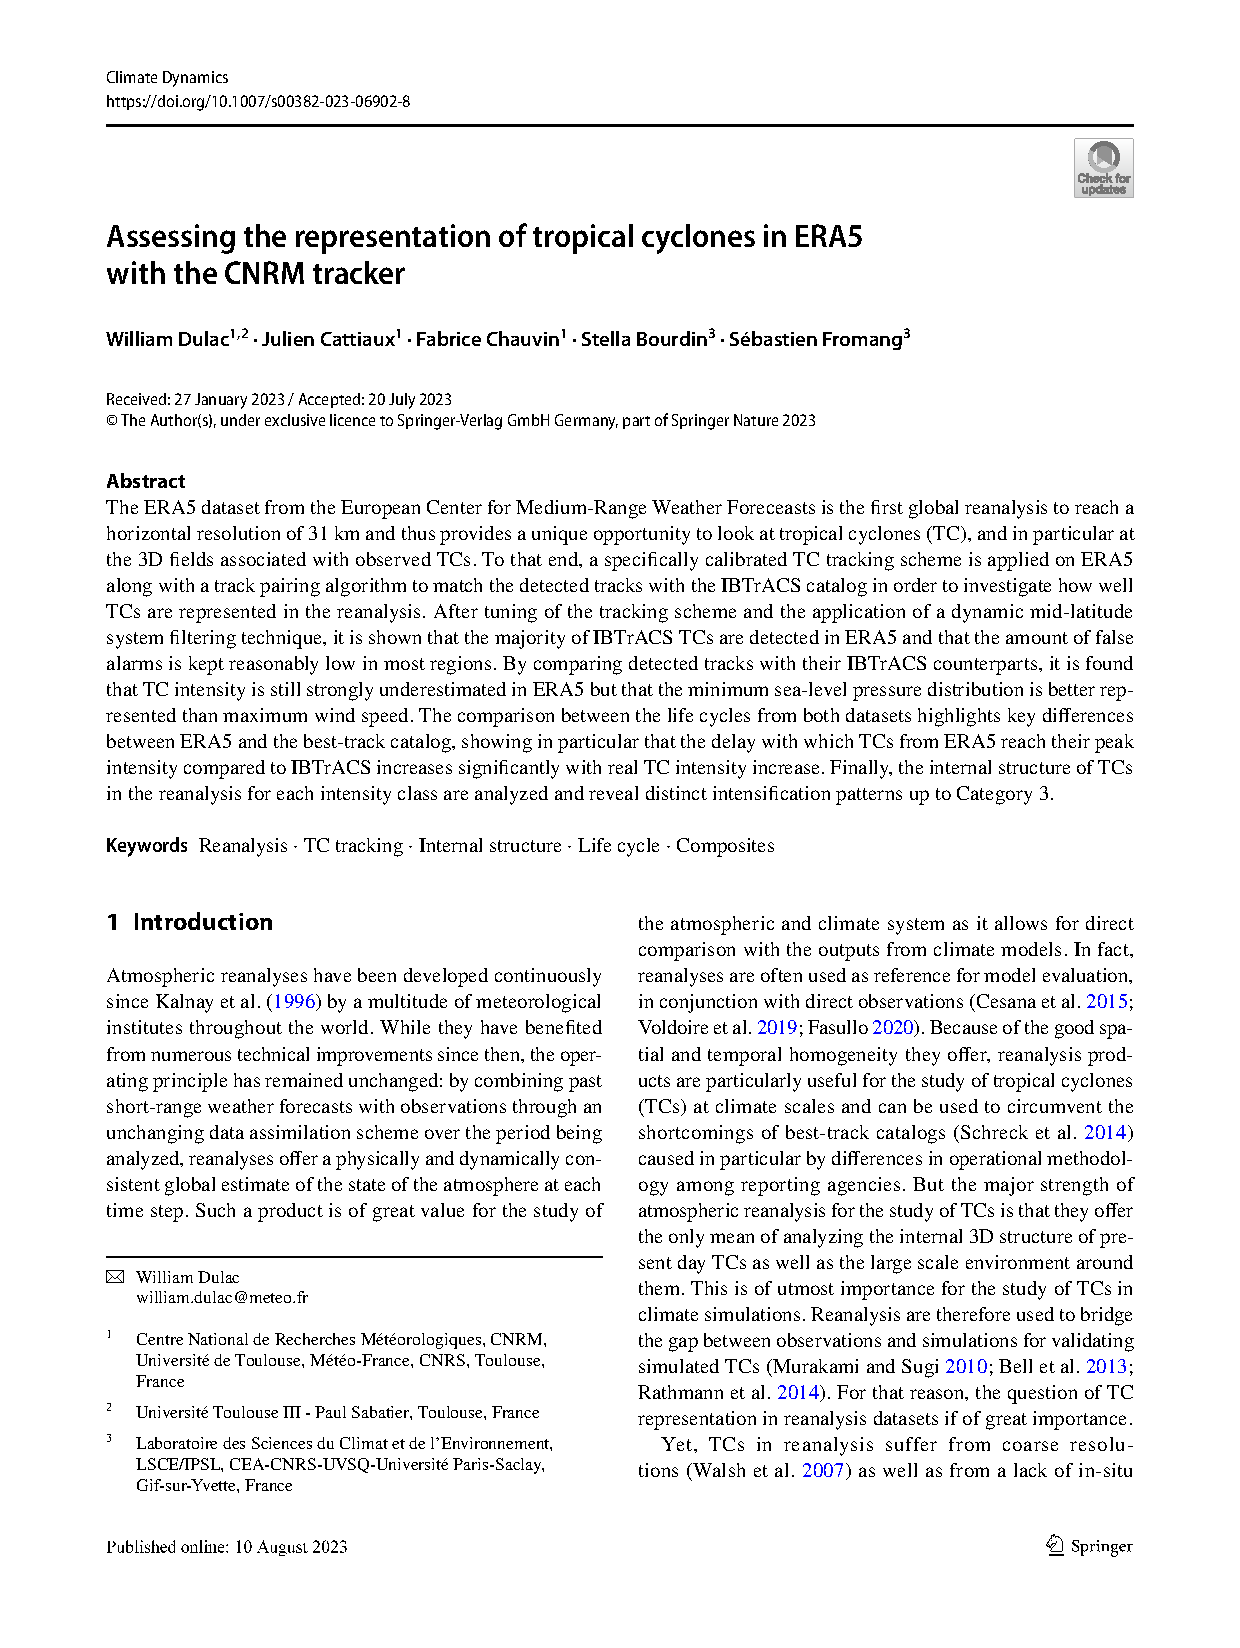
\includepdf[pages=-,pagecommand={\thispagestyle{plain}},offset=5mm 0mm,frame=false,noautoscale=true,scale=1,addtotoc=
    {1,section,1,Article Climate Dynamics,sec:papier,
     1,subsection,2,Introduction,sec:papier_intro,
     2,subsection,2,Données et méthodes,sec:papier_data_methods,
     3,subsubsection,3,Algorithme de détection du CNRM,sec:papier_cnrm_tracker}]{\subfix{../include/dulac2023.pdf}}

\section{Compléments}

\subsection{Filtrage des systèmes de moyennes latitudes}\label{sec:filtrage_mid_latitudes}

\subsection{Métriques d'évaluation de la similarité des trajectoires}

%--------------------------------------
\section{Synthèse}

\end{document}
